\section{\aintranet\ des maisons d'édition \aey}
\label{eyrolles}

Ce projet est celui pour lequel j'ai consacré la majeure partie de mon stage. Les sections suivantes décrivent le contexte et les objectifs du projets (section~\ref{section:eyrolles_contexte}), ma place dans l'organisation du travail (section~\ref{section:eyrolles_organisation}) puis les fonctionnalités attendues de l'application (section~\ref{section:eyrolles_fct}). Les sections~\ref{section:eyrolles_modules}, \ref{section:eyrolles_webservices}, \ref{section:eyrolles_tests} et \ref{section:eyrolles_prod} rentrent dans le détail de quelques points techniques. Quant à la dernière section~\ref{section:eyrolles_bilan}, elle est consacrée à mon bilan d'expérience.


\subsection{Contexte et objectifs}
\label{section:eyrolles_contexte}

Le groupe \aey\ est un groupe français d'édition spécialisé dans les domaines du livre professionnel et technique, et publie notamment des livres consacrés à l'informatique.

Historiquement, \aey\ gérait l'ensemble de ses données par le biais de documents sous format papier, d'autres sous format numérique (documents \amsword, \amsexcel\ldots), ainsi que des \aemails. Utiliser de tels supports en tant que base de référence pour l'ensemble des processus métiers engendre des inconvénients majeurs :

\begin{itemize}
	\item les mêmes informations sont ressaisies plusieurs fois dans les documents ;
	\item les informations ne sont pas toujours saisies de la même manière ;
	\item la mise à jour des informations n'est pas toujours répercutée partout ;
	\item l'information circule sous des formats hétérogènes, d'où une difficulté de réutilisation.
\end{itemize}

\aey\ a alors pris la décision de constituer une véritable base d'information accessible sous la forme d'un \aintranet\ par les acteurs des différents services. Une partie de ce projet a été mis en production sous l'appellation de \emph{\alotun}. Celle-ci propose une base de données produits, associée entre autres aux fonctionnalités suivantes :

\begin{itemize}
	\item la gestion des processus métiers spécifiques au service commercial ;
	\item la création de documents, à partir de modèles prédéfinis, permettant de créer des documents commerciaux ;
	\item l'export d'information en fonction de critères choisis par l'utilisateur (format, type d'informations).
\end{itemize}

Exploité depuis mars~2007, ce \alotun\ est en constante évolution.

Dans la continuité, le groupe \aey\ souhaite étendre l'\aey\ afin de disposer d'une base de projets éditoriaux commune, fiable et accessible par l'ensemble des services. Cette nouvelle base serait associée à une interface de gestion et de suivi des processus d'édition, de fabrication, de commercialisation et de
promotion des livres.

L'agence web \asl\ a alors été choisie en tant que prestataire pour analyser puis implémenter ce nouveau projet, intitulé \emph{\alotdeux}.


\subsection{Organisation du travail}
\label{section:eyrolles_organisation}

Pour ma part, j'ai été affecté en tant que développeur sur le projet \aey. J'ai pu travailler avec \acohen, le chef de projet, ainsi que les développeurs \ahamon, \aweistroff\ et \abachelet. 

Cette section décrit les différentes phases du projet \aey\ et reprend son planning.


\subsubsection{Planning}

Le planning tel qu'il a été établi au début du projet est le suivant :

\begin{description}
	\item[Phase de développement] du 21 septembre 2009 au 11 décembre 2009 ;
	\item[Phase de recette] du 14 décembre 2009 au 8 janvier 2010 ;
	\item[Livraison finale] le 11 janvier 2010.
\end{description}

Le planning réel a pris du retard sur le planning initial :

\begin{description}
	\item[Phase de développement] du 21 septembre 2009 au 11 décembre 2009 ;
	\item[Phase de recette] du 14 décembre 2009 au 17 février 2010 ;
	\item[Livraison finale] le 18 février 2010.
\end{description}

Note : les phases de spécification et d'analyse ne sont pas listées dans le planning du fait que je n'étais pas encore arrivé chez \asl\ quand elles ont eu lieu.


\subsubsection{Phase de spécification}

Conjointement avec le client, \acohen\ s'est chargé de la rédaction du cahier des charges du projet. Il en ressort un dossier d'une centaine de pages, décrivant les fonctionnalités attendues, les règles métiers ou encore des prototypes d'interface utilisateur. C'est ce document qui a servi de fil rouge tout au long de la réalisation du projet.


\subsubsection{Phase d'analyse}

La phase d'analyse du projet a consisté à mettre en place le modèle de l'application sous la forme d'un diagramme, le \amcd\footnote{Le \amcd, ou Modèle Conceptuel de Données, établit sous forme de diagramme une représentation des données et définit les dépendances fonctionnelles entre elles.}. À l'\autc, nous avons eu l'occasion de réaliser des \amcds\ dans l'\auv\ NF17\footnote{Cours de conception de bases de données à l'\autc.} en utilisant le format \auml\footnote{\auml\ (\textit{Unified Modeling Language}) est un langage de modélisation graphique standardisé utilisé dans le domaine du génie logiciel, notamment dans le cadre de la conception orientée objet.~\cite{uml}} ou \aea\footnote{Le modèle entité-association, ou modèle \aea, est une représentation abstraite et et conceptuelle de données. Il est notamment utilisé pour modéliser des schémas de base de données.~\cite{ea}}. Chez \asl, les diagrammes \amcds\ sont réalisés au format \aea\ et sont réalisés à l'aide de l'outil \amysqlwb.

Le \amcd\ du \alotdeux\ d'\aey, modélisé par \acohen\ et \ahamon, comprend de nombreuses tables et de nombreux liens. Pour gagner en lisibilité, les tables et les liens n'ont pas tous été représentés : seuls les plus importants permettant de mieux comprendre le fonctionnement de l'application ont été choisis.


\subsubsection{Phase de développement}

Ma participation au projet \aey\ a commencé au début de la phase de développement. Avec \ahamon, nous y avons développé la plupart des fonctionnalités attendues\footnote{Cf. section~\ref{section:eyrolles_fct}}. Début décembre, \aweistroff, qui venait d'être embauché par \asl, nous a rejoint pour soutenir le rythme d'implémentation.

La répartition du travail s'est mise en place simplement en affectant, au fur et à mesure de l'avancement du projet, une fonctionnalité à implémenter à chaque développeur. Chaque fonctionnalité à traiter a été choisie par le chef de projet en fonction de sa priorité estimée. Le code source de l'application était partagé via un dépôt \asvn\footnote{Cf. section~\ref{section:outils_svn}}.

Le \alotdeux\ de l'\aintranet\ d'\aey\ utilise la version 1.3 de \asf. Au moment où le développement du projet avait commencé, cette version du \afm\ n'était pas encore sortie en version finale et était encore en plein développement. Comme c'est \asl\ qui est à l'origine de \asf, la maîtrise sur le \afm\ en interne est importante : l'entreprise peut donc se permettre d'utiliser les dernières technologies disponibles.

Les contraintes techniques de développement imposent d'utiliser une base de données \apsql, à la demande du client. L'utilisation de \asf\ 1.3, quant à elle, nécessite une version de \aphp\ supérieure à 5.2.4. Le serveur \ahttp\ utilisé est \aapache~2.


\subsubsection{Phase de recette}
\label{section:eyrolles_organisation_recette}

La phase de recette consiste à faire tester l'application au client, qui va pouvoir faire remonter les éventuels \abugs\ à corriger ou les fonctionnalités à améliorer. La communication entre le client, le chef de projet et les dé\-ve\-lop\-peurs s'est déroulée via le système de gestion de projet \atrac\footnote{Cf. section~\ref{section:outils_trac}}.

En fait, le client y rédige la description de son \abug\ dans un ticket. Le chef de projet le valide, et l'assigne ensuite au développeur qui doit s'en charger. Une fois que le développeur a fait son travail d'implémentation sur un ticket, il le renvoie au chef de projet qui vérifie la fonctionnalité modifiée. Si tout se passe bien, le ticket est retourné à nouveau au client pour qu'il se rende compte par lui-même de l'amélioration. Le client satisfait clôt alors le ticket ; dans le cas contraire, il initie un nouveau cycle d'échange sur celui-ci. Ce processus de recette via rapports de \abugs\ est illustré dans la figure~\ref{figure:eyrolles_organisation_tickets}.

\begin{figure}
	\centering
	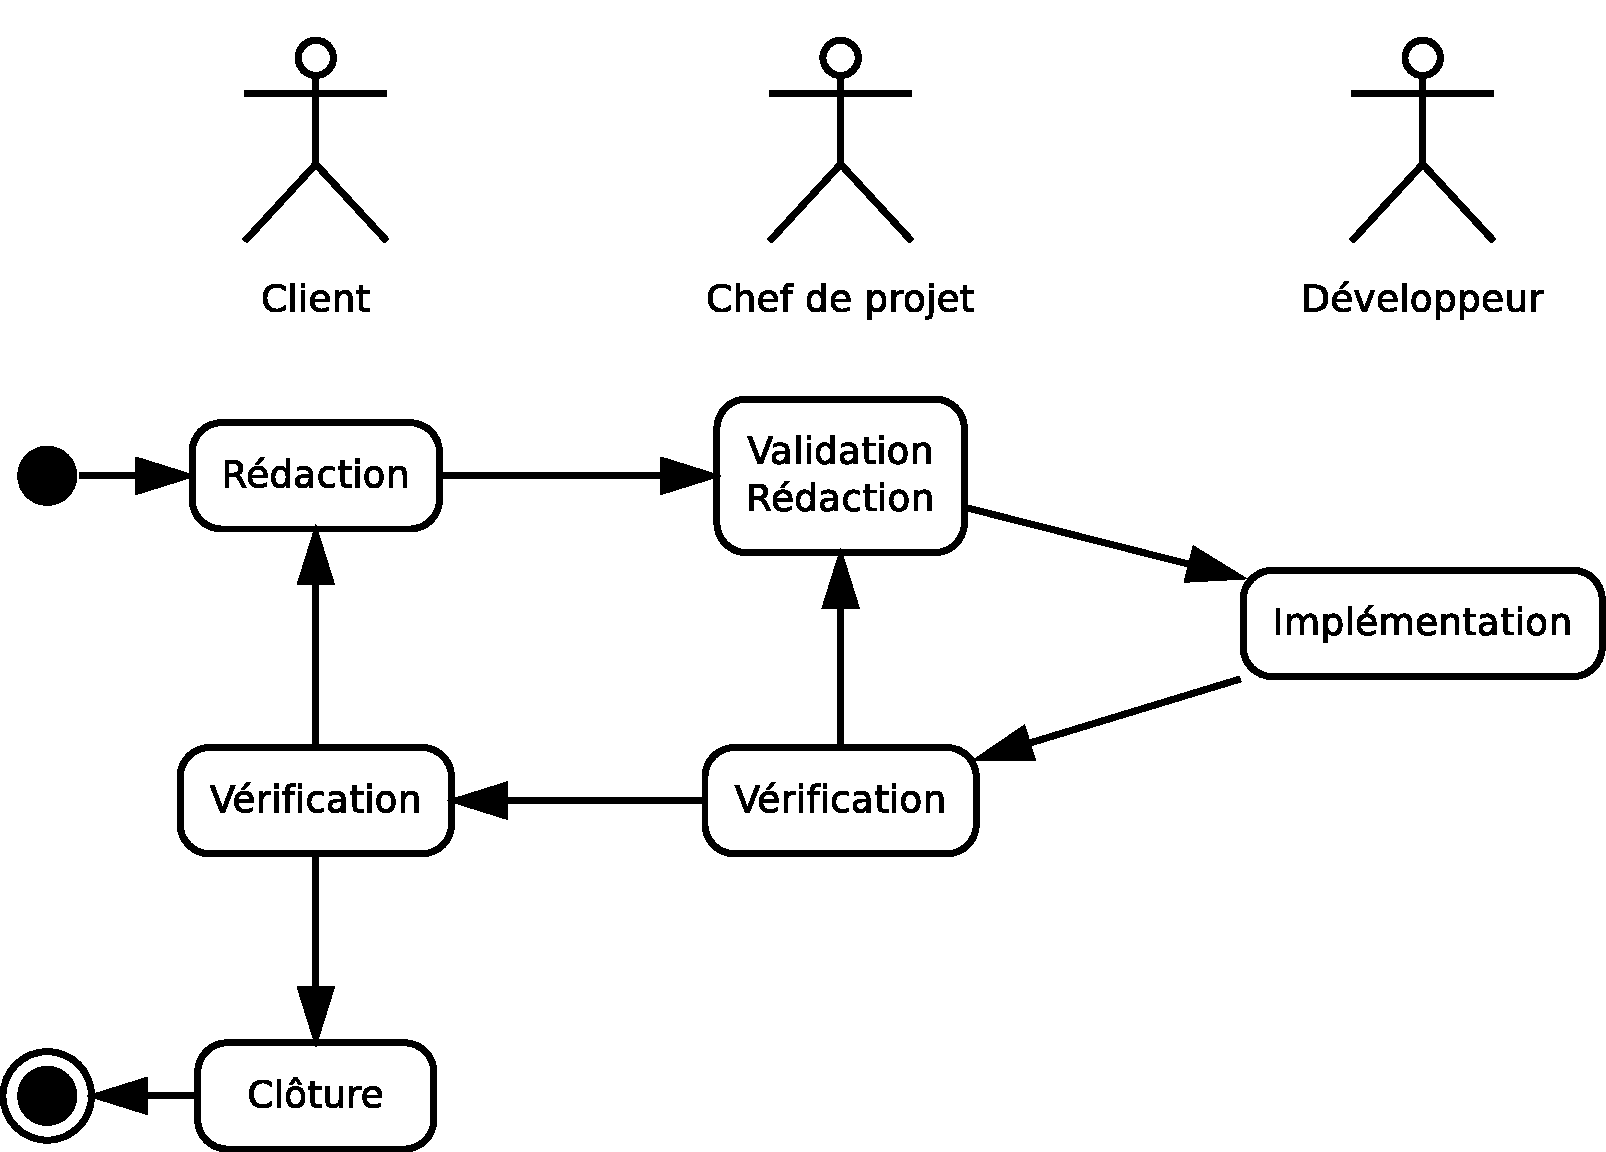
\includegraphics[scale=0.4]{eyrolles_organisation_tickets}
	\caption{États d'un ticket dans le cas du processus de recette d'\aey}
	\label{figure:eyrolles_organisation_tickets}
\end{figure}

Par ailleurs, pour permettre au client de tester correctement l'application, il est nécessaire de lui montrer régulièrement les nouvelles versions du projet. Cette démarche s'est traduite par une livraison hebdomadaire de l'application sur le serveur du client. Le processus de livraison d'\aey\ est décrit plus tard dans la section~\ref{section:eyrolles_prod}.

Du point de vue de l'organisation du travail, \ahamon\ a quitté l'équipe de développement d'\aey\ au moment du passage en phase de recette, afin de s'occuper du pôle formation de \asl. Pendant trois semaines, j'ai continué avec \aweistroff, qui a ensuite été affecté sur un autre projet début janvier. J'ai continué pendant quelques temps à développer seul sur le projet, et fin janvier, \abachelet\ m'a rejoint ponctuellement pour m'aider à fermer les tickets restants.


\subsubsection{Livraison finale}

La livraison finale ayant été repoussée après mon départ, je n'aurais pas eu l'occasion d'y participer. Toutefois, le processus sera exactement le même que celui utilisé durant la phase de recette.


\subsection{Fonctionnalités attendues de l'\aintranet}
\label{section:eyrolles_fct}

Cette section offre un aperçu des fonctionnalités commandées par le client, qui ont été rassemblées dans le cahier des charges du projet au moment de la phase de spécification.

Comme il l'a été annoncé dans la section~\ref{section:eyrolles_contexte}, le but principal du \alotdeux\ de l'\aintranet\ d'\aey\ est de fournir une base des projets éditoriaux de la maison d'édition. Le projet est donc l'objet central de l'application. Il peut représenter différents types d'œuvre : un livre, un \advd, un \aebook\footnote{Un \aebook, ou livre électronique, est un texte numérisé pouvant être lu sur un support électronique.~\cite{ebook}}, ou encore un couple livre + \aebook. Chaque projet s'identifie par son code \ageodif, qui est en fait le code commercial interne à \aey. À partir de cet identifiant peuvent être générés des codes plus classiques et plus répandus, comme l'\aisbn\ ou l'\aean.

L'ensemble des fonctionnalités de l'\aintranet\ est soumise à un contrôle d'accès utilisateur. En effet, un utilisateur de l'application web devra se connecter à l'aide d'un identifiant et d'un mot de passe, tous deux enregistrés dans la base de données. Il lui est attribué un rôle utilisateur, comme \og invité \fg, \og éditeur \fg\ ou encore \og administrateur \fg\ par exemple, qui définit un ensemble de permissions. Ainsi, l'utilisateur identifié se verra autoriser ou refuser des accès en fonction du rôle qui lui a été affecté initialement. Par soucis d'ergonomie, toutes les fonctionnalités dont l'utilisateur n'a pas accès lui sont cachées.

Les fonctionnalités attendues sont listées ci-après, celles que j'ai moi-même développées étant marquées d'une astérisque :

\begin{itemize}
	\item gestion de la session utilisateur :
    	\begin{itemize}
			\item profil utilisateur ;
			\item synchronisation \aldap\footnote{\aldap\ (\textit{Lightweight Directory Access Protocol}) est un protocole reposant sur \atcpip\ permettant l'interrogation et la modification de services d'annuaire.~\cite{ldap}} des comptes utilisateurs ;
			\item rôles utilisateur et permissions ;
			\item contrôles d'accès ;
		\end{itemize}
    \item modules relatifs au projet :
    	\begin{itemize}
			\item onglet \og tableau de bord \fg ;
			\item onglet \og informations générales \fg ;
			\item onglet \og intervenants externes \fg ;
			\item onglet \og devis \fg ;
			\item onglet \og fiche projet \fg ;
			\item onglet \og validations \fg ;
			\item onglet \og \abat\ \aef\ \fg\aast\ (formulaire de processus métier) ;
			\item onglet \og dépôt de documents \fg ;
			\item onglet \og résumés \fg ;
			\item onglet \og fabrication \fg ;
			\item création de projets de types \og nouveauté \fg, \og nouvelle édition \fg, \og \textit{relookage} \fg, \og réimpression \fg, \og tirage spécial \fg\aast ;
			\item historique d'une œuvre ;
			\item déclenchement d'étapes de processus métier : validation, \aomf\footnote{Ordre de Mise en Fabrication}, \aomr\footnote{Ordre de Mise en Réimpression}, \aoet\footnote{Ordre d'Envoi en Tirage}, référencement\aast, clôture ;
			\item listing des projets\aast, des demandes de validation projet\aast, des demandes de déclenchement \aoet\aast, du planning \aef\aast ;
		\end{itemize}
	\item module de gestion des intervenants externes\aast\ (auteurs, contacts, prestataires) ;
	\item module de gestion des collections d'œuvres ;
	\item modules de gestion des maisons d'éditions\aast\ (internes à \aey\ ou externes) ;
	\item module de gestion des codes \ageodif\aast ;
	\item module de gestion des contrats ;
	\item module de gestion des demandes de paiement ;
	\item module de gestion des relevés de travaux ;
	\item module du panier de projets d'un utilisateur\aast, avec export de documents\aast\ au format \azip\footnote{Le \azip\ est un format de fichier permettant l'archivage et la compression de données sans perte de qualité.~\cite{zip}} et export de données\aast\ au format \acsv\footnote{\acsv\ (\textit{Comma-Separated Values}) est un format informatique ouvert  représentant des données tabulaires sous forme de \og valeurs séparées par des virgules \fg.~\cite{csv}} ;
	\item modules de référentiels\footnote{Un référentiel est un ensemble de bases de données contenant les \og références \fg\ d'un système d'information.~\cite{referentiel}} administrables divers\aast :
		\begin{itemize}
			\item marques utilisées sur une œuvre ;
			\item natures de contribution des intervenants externes ;
			\item natures des prestations ;
			\item spécialités de prestataires ;
			\item langues ;
			\item types d'intérieurs de livres ;
			\item types de couvertures ;
			\item types d'embellissements (mat, brillant\dots) ;
			\item types de produits complémentaires (\acd, \advd\dots) ;
			\item types de contrats ;
			\item motifs de clôture de projets ;
			\item formats \aebook ;
		\end{itemize}
	\item \awss\ de communication avec le \alotun\aast\ (voir la section~\ref{section:eyrolles_webservices}) ;
	\item tâches exécutables via la ligne de commande\aast :
		\begin{itemize}
			\item initialisation des auteurs, des collections et des thématiques via les \awss\ associés ;
			\item initialisation des codes \ageodif\ via un fichier \acsv ;
			\item mise à jour des statuts des projets, des informations commerciales des projets.
		\end{itemize}
\end{itemize}

Ce \alotdeux\ de l'\aintranet\ d'\aey\ est donc un projet conséquent qui justifie bien l'implication de plusieurs développeurs.


\subsection{Fonctionnement des modules de l'application}
\label{section:eyrolles_modules}

Le \afm\ \asf\ oblige le développeur à construire son application web en la divisant sous forme de modules. Généralement, chaque module regroupe un ensemble de pages (nommées \emph{actions}) partageant un domaine fonctionnel commun. Cette bonne pratique favorise la maintenabilité et la lisibilité du code.

En effet, dans \aey, on compte une quarantaine de modules, comme \texttt{ey\-Referential\-Language} ou \texttt{eyContract}, gérant respectivement le ré\-fé\-ren\-ti\-el des langues et les contrats. Le module des contrats, par exemple, contient des pages comme celle listant les contrats ou encore celle permettant d'en créer.

Par rapport à ceux d'une application web lambda développée en \asf, les modules de l'\aintranet\ d'\aey\ ont la spécificité de se baser sur \asladmin\ et d'avoir subi une factorisation supplémentaire.


\subsubsection{Utilisation de \asladmin}

La plupart des vues du \alotdeux\ de l'\aintranet\ d'\aey\ sont générées grâce au \aplugin\ \asf\ \asladmin. Il a été développé en interne par \asl\ et est issu de l'abstraction du code d'un précédent projet. Il n'a rien à voir avec la fonctionnalité de génération d'administration intégrée à \asf. C'est encore un \aplugin\ très jeune : \aey\ est le premier projet qui l'utilise.

Le \aplugin\, tout comme la génération d'administration, permet de ne pas avoir à redévelopper la logique des opérations de base, telles que le listing d'éléments, sa pagination, son tri, ou encore la création, l'édition et la suppression d'éléments. Sa valeur ajoutée est qu'il apporte plus de flexibilité quant à la personnalisation de la logique et des différentes vues. Le tableau~\ref{table:eyrolles_sladmin_sladmin-vs-admin-gen} reprend une comparaison rapide des différences entre le moteur de génération d'administration de \asf\ et \asladmin.

\begin{table}
	\centering
	\begin{tabular}{|p{3cm}||p{4.5cm}|p{4.5cm}|}
		\hline
		& Génération d'administration & \asladmin\ \tabularnewline
		\hline
		\hline
		Format de configuration & \ayml & code \aphp \tabularnewline
		\hline
		Génération de code & oui & non \tabularnewline
		\hline
		Personnalisation de la logique & surcharge de code généré & surcharge d'actions de base \tabularnewline
		\hline
		Personnalisation des vues & surcharge de vues générées & écriture classique de vues \tabularnewline
		\hline
	\end{tabular}
	\caption{Comparaison entre la génération d'administration de \asf\ et \asladmin}
	\label{table:eyrolles_sladmin_sladmin-vs-admin-gen}
\end{table}

Ainsi, \asladmin\ permet de gagner du temps de développement et d'assurer une factorisation des opérations récurrentes d'administration du site.


\subsubsection{Agencement des modules}

Habituellement, les actions un module \asf\ reposent directement sur les classes d'actions de base intégrées au \afm. Ce comportement est nécessaire pour que les actions puissent d'exécuter et engendrer l'affichage des pages correspondantes.

L'utilisation de \asladmin\ change la donne : elle nécessite de baser les actions du module sur les classes d'actions propres au \aplugin, qui elles-mêmes se basent sur celles de \asf. Les classes d'actions de \asladmin\ intègrent les actions génériques décrites plus tôt, comme par exemple celles permettant de lister, créer ou supprimer des éléments.

La modélisation de l'\aintranet\ d'\aey\ est allée encore plus loin, en intégrant une nouvelle couche d'actions propres au projet entre celles des modules et celles de \asladmin. Son but est de permettre de modifier le comportement des actions de \asladmin\ afin qu'elles correspondent au mieux aux besoins du projet, sans pour autant avoir besoin de modifier le \aplugin.

Finalement, en plus d'être organisée horizontalement sous forme de modules, l'application est également découpée verticalement en différentes cou\-ches. Ses différentes fonctionnalités ont alors l'avantage de se distinguer les unes des autres, tout en partageant à la fois des bases communes. Cette organisation est illustrée dans la figure~\ref{figure:eyrolles_modules_couches}.

\begin{figure}
	\centering
	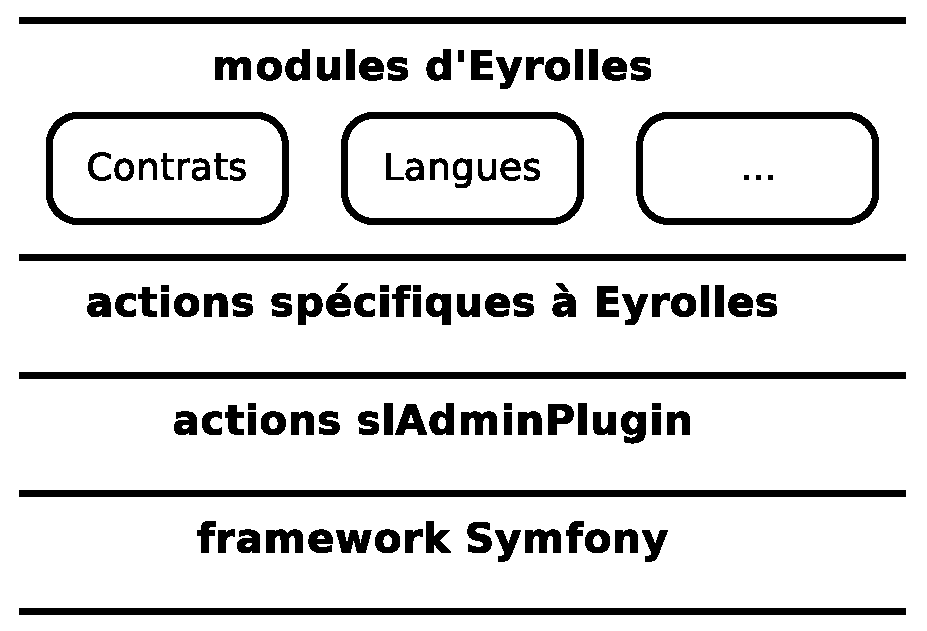
\includegraphics[scale=0.4]{eyrolles_modules_couches}
	\caption{Organisation des modules du \alotdeux\ d'\aey}
	\label{figure:eyrolles_modules_couches}
\end{figure}

\subsection{Modélisation des \awss}

La fonctionnalité des \awss\ annoncée en partie~\ref{section:eyrolles_fct} se résume à permettre à l'application développée, le \alotdeux, de communiquer avec la partie de l'\aintranet\ déjà existante, le \alotun.

Techniquement, un \aws\ est une interface (\aapi) accessible via un réseau et qui permet d'exécuter des actions sur un système distant. Dans le cas d'\aey, c'est le \alotdeux\ qui utilise l'interface du \alotun\footnote{Les \awss\ du \alotun\ sont développés en interne chez \aey.}, et jamais l'inverse. Les \awss\ du \alotdeux\ consistent alors à envoyer des données dans le bon format aux \awss\ du \alotun, et éventuellement de recevoir une réponse. Les données sont échangées via le protocole \ahttp, et le format de données utilisé est le \ajson\footnote{JSON (JavaScript Object Notation) est un format de données textuel permettant de représenter de l'information structurée.\\Exemple : \texttt{\{"auteur": \{"id": "1", "nom": "Jean Dupont"\}\}}}. La figure~\ref{figure:eyrolles_webservices_echange} illustre la façon dont les lots indépendants de l'\aintranet\ d'\aey\ communiquent.

\begin{figure}
	\centering
	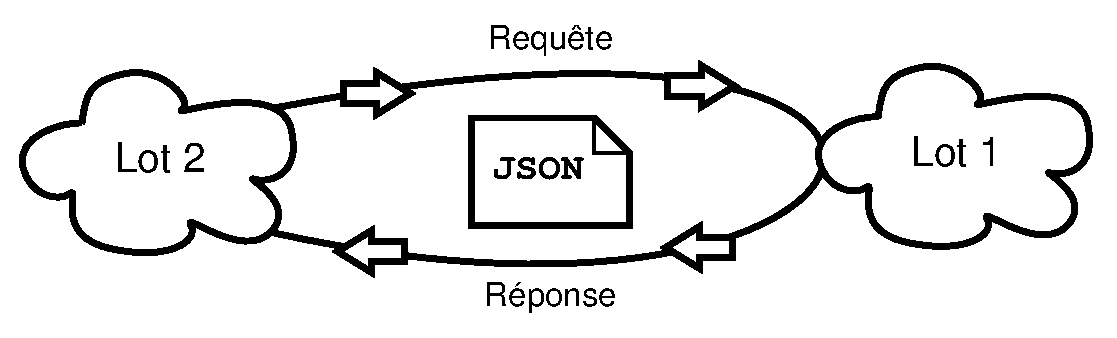
\includegraphics[scale=0.6]{eyrolles_webservices_echange}
	\caption{Principe de communication via \aws\ entre le \alotun\ et le \alotdeux\ d'\aey}
	\label{figure:eyrolles_webservices_echange}
\end{figure}

Les \awss\ à développer sur le \alotdeux\ sont les suivants :

\begin{itemize}
	\item le \aws\ des auteurs (initialisation et mise à jour) ;
	\item le \aws\ des collections (initialisation et mise à jour) ;
	\item le \aws\ des thématiques (initialisation) ;
	\item le \aws\ de demande de référencement ;
	\item le \aws\ de mise à jour des statuts de projets ;
	\item le \aws\ de mise à jour des informations commerciales des projets.
\end{itemize}

Tous ces types de \aws\ diffèrent en fait par l'adresse à laquelle ils doivent envoyer leur requête et par les paramètres qu'ils doivent fournir. Le processus d'échange de données avec le \alotun, quant à lui, est commun à tous. Le système à implémenter doit donc être modélisé, afin d'éviter d'écrire du code redondant et de faciliter une maintenance ultérieure. Cette étape de modélisation est une tâche clé du travail d'ingénieur, dans le sens où elle est nécessaire pour anticiper une évolution pérenne d'un système.

Le diagramme \auml\ de la figure~\ref{figure:eyrolles_webservices_uml} reprend la modélisation qui a été effectivement choisie.

\begin{figure}
	\centering
	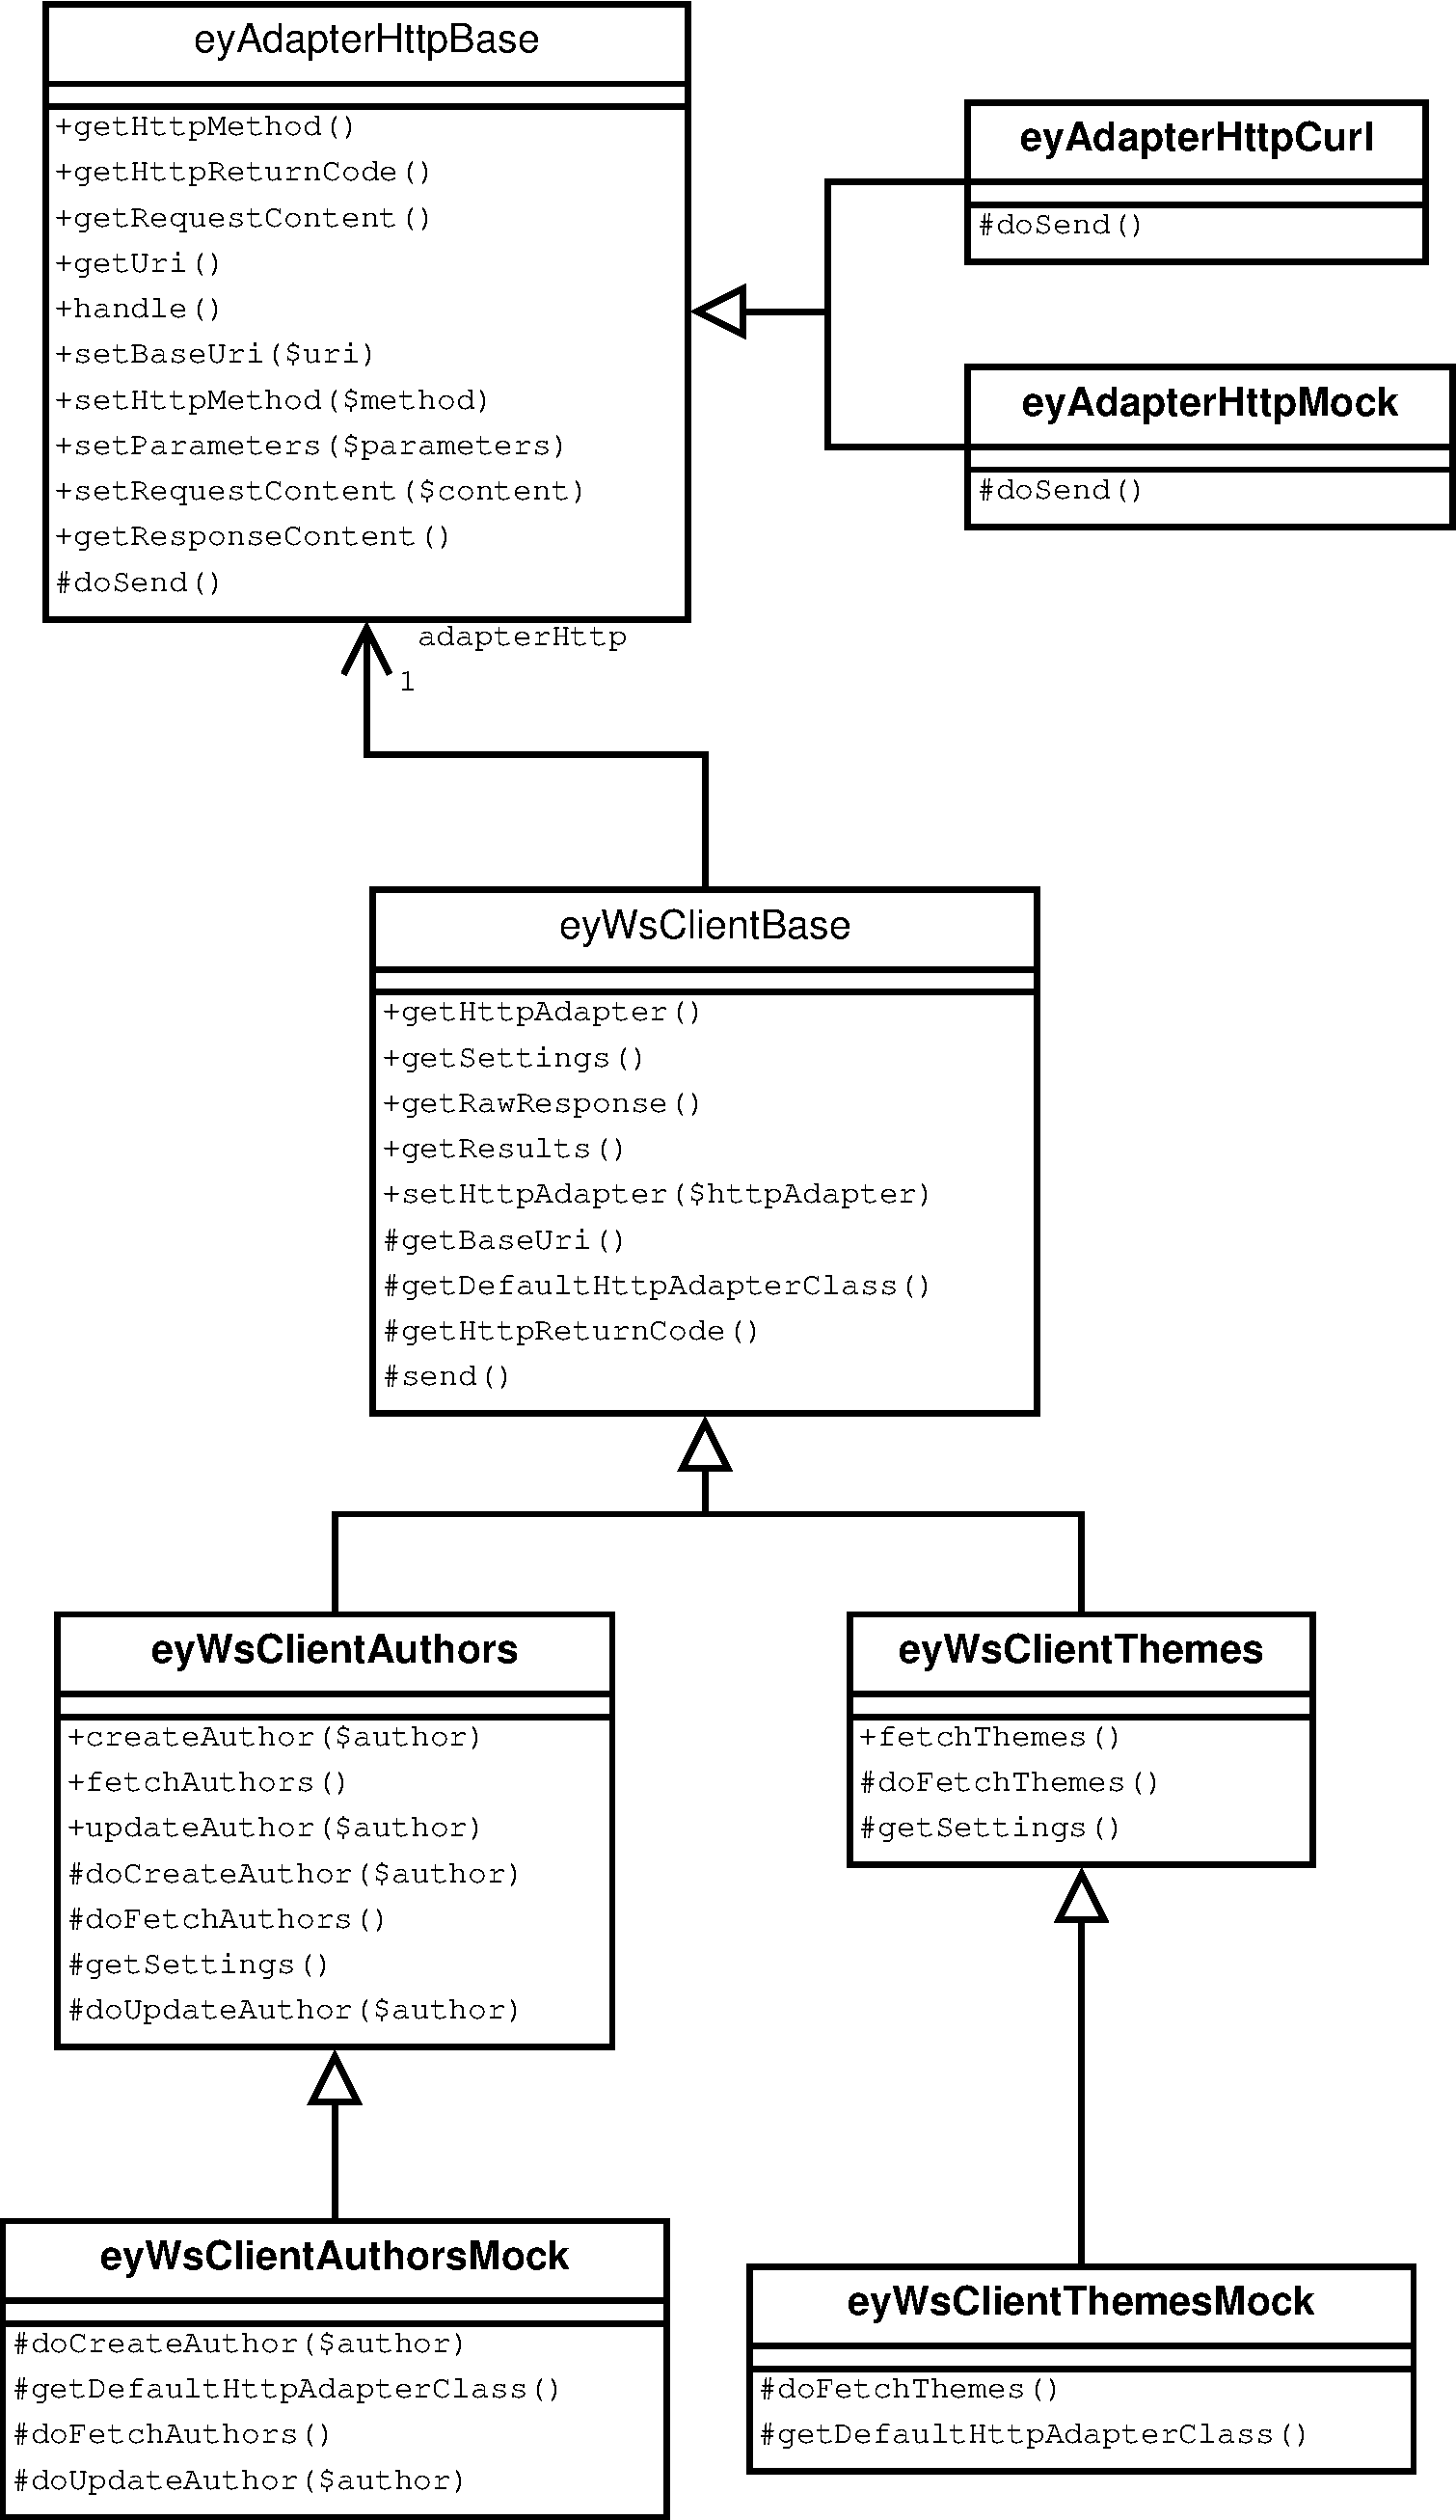
\includegraphics[scale=0.4]{eyrolles_webservices_uml}
	\caption{Modélisation des classes de \aws}
	\label{figure:eyrolles_webservices_uml}
\end{figure}

En effet, l'ensemble du code concernant la procédure de communication a été factorisé dans une classe \texttt{eyWsClientBase}. Les classes qui héritent de celle-ci, comme \texttt{eyWsClientAuthors} ou \texttt{eyWsClientThemes}, représentent les différents types de \aws. Au final, ces classes filles ne contiennent que les méthodes consistant à définir quels paramètres doivent être envoyés dans la requête, ou encore comment retourner la réponse à l'application.

Par ailleurs, l'implémentation de la liaison \ahttp\ a été isolée des classes de \aws\ : la classe abstraite \texttt{eyAdapterHttpBase} regroupe l'ensemble des méthodes permettant de stocker la méthode \ahttp\ à utiliser, les paramètres à envoyer ou encore l'adresse distante à consulter. Le contact effectif du \aws\ distant s'effectue dans la méthode \texttt{doSend()} surchargée dans les classes filles, telles que \texttt{eyAdapterHttpCurl} par exemple. Chaque classe \texttt{eyWsClient*} fait alors appel à une classe \texttt{eyAdapterHttp*} qui va se charger d'envoyer les données via le protocole \ahttp.

L'intérêt d'avoir différentes classes héritant de \texttt{eyAdapterHttpBase} permet de pouvoir implémenter de différentes façons l'appel au \aws\ distant. En effet, sur \aey, ce sont les fonctions de l'extension \acurl\footnote{La libraire \acurl\ donne la possibilité de récupérer, de créer ou encore de modifier le contenu d'une ressource accessible par le réseau, et supporte nottamment le protocole \ahttp.} de \aphp\ qui sont utilisées. En imaginant que l'\aintranet\ d'\aey\ soit déplacé sur un serveur sur lequel l'extension n'est pas installée, il serait très facile de réécrire une classe alternative, comme \texttt{eyAdapterHttpStream} qui utiliserait les fonctions \texttt{stream} disponibles en natif.

En outre, quand un développeur teste l'application du \alotdeux\ avec des données factices, il n'est pas concevable que celles-ci soient effectivement envoyées au \alotun\ pour le mettre à jour, au risque de corrompre l'intégrité des données de production. Il est donc nécessaire de prévoir une façon de simuler l'appel à un \aws.

Par exemple, dans le cas du \aws\ des auteurs, une classe \texttt{ey\-Ws\-Client\-Authors\-Mock} hérite de la classe \texttt{eyWsClientAuthors}. Entre autres, elle redéfinit la méthode sensée envoyer une requête de mise à jour d'un auteur au \alotun\ et ne fait rien à la place. Il est ainsi aisé de redéfinir des comportements initiaux, une fois que le problème a été modélisé en faisant appel aux grands principes de la programmation orientée objet.


\subsection{Écriture de tests}

Le projet \aey\ n'échappe pas à la règle : comme ses pairs, il est lui aussi soumis, via \asismo, au processus d'intégration continue décrit dans la partie~\ref{section:sismo}.

Le \afm\ \asf\ supporte deux types de tests : les tests unitaires et les tests fonctionnels.


\subsubsection{Tests unitaires}

\begin{quote}
Le test unitaire est un procédé permettant de s'assurer du fonctionnement correct d'une partie déterminée d'un logiciel ou d'une portion d'un programme.\cite{unit}
\end{quote}

Avec \asf, la bonne pratique consiste à tester les méthodes des classes de modèle et des classes utilitaires, indépendamment du reste de l'application. En effet, si à un moment ou un autre un des développeurs modifie le comportement de l'une des méthodes clés testées, les tests unitaires concernés deviendront potentiellement invalides.

Deux cas sont alors possibles : soit le nouveau comportement est désiré, soit au contraire c'est une erreur. Dans le premier cas, les tests unitaires ainsi que les parties de l'application qui utilisent leurs spécifications doivent être modifiés en conséquence. Dans le second, le comportement doit revenir dans son état précédent alors que les tests restent intacts. Dans chaque situation, le but est de ramener la suite de tests vers son état valide. Ainsi, l'écriture de tests unitaires est une bonne façon de s'assurer que toute modification de code testé sera suivie d'une vérification.

Une façon de tester unitairement une méthode consiste à l'appeler plusieurs fois, avec des paramètres ou un contexte différent. On vérifie alors si les valeurs retournées sont bien celles attendues, si une exception est propagée, si le contexte est de le bon état, etc.

Dans \asf, les tests unitaires sont effectués à l'aide du \afm\ de test unitaire \alime, développé pour \asf. Sur le projet \aey, ils ont été écrits tout au long du cycle de développement. Par souci de pragmatisme, seules les méthodes relativement importantes sont testées : il s'agit de ne pas perdre de temps avec les méthodes évidentes, ce qui reviendrait à tester les fonctionnalités de \asf\ elles-mêmes déjà unitairement testées de leur côté.

Par ailleurs, certaines fonctionnalités du projet à la logique poussée ont été développée en utilisant la méthode Test driven development (TDD), soit le développement 

Au delà de prévenir les régressions sur le projet, l'écriture de tests unitaires a permis de mettre à l'épreuve rapidement chaque mé


\subsubsection{Tests fonctionnels}

TODO

\subsection{Processus de mise en production}
\label{section:eyrolles_prod}

TODO


\subsection{Bilan}
\label{section:eyrolles_bilan}

Travailler sur un projet aussi conséquent que celui de l'\aintranet\ d'\aey\ a été pour moi très instructif. En effet, il m'a permis de me confronter à de nombreuses problématiques du développement web.

Je me suis rendu compte que travailler à plusieurs développeurs sur un chantier d'une telle envergure n'était pas aussi facile que ce que j'imaginais. Déjà bien habitué au partage de code source via les systèmes de gestion de versions comme \asvn, je considérais que ces outils étaient la réponse à tous les problèmes de travail en équipe. Au-delà des simples conflits de fichiers modifiés par plusieurs parties au même instant, j'ai pu faire l'expérience de problèmes liés à la communication au sein de l'équipe de développement. Par exemple, il nous est arrivé de faire le lien entre deux tables de la base de données de trois façons différentes : chaque développeur avait implémenté la fonctionnalité à sa façon. Une solution est de ne jamais hésiter à faire le point avec ses collègues, et de régulièrement se lister l'ensemble des points que chacun a traité.

Par ailleurs, avec le recul, nous nous sommes rendus compte que l'utilisation de \asladmin\ en tant que base de chacun de nos modules n'était pas une si bonne idée. Pendant toute la première partie de la phase de développement, ce \aplugin\ nous a effectivement fait gagner du temps. Nous avons commencé à ressentir ses faiblesses quand il s'agissait de gérer des modules plus complexes : le développement devenait plus compliqué que ce qu'il l'aurait été sans utiliser \asladmin. En fait, le gros point négatif nous est apparu quand de nouveaux développeurs sont arrivés dans un deuxième temps sur le projet : ils se sont sentis relativement perdus et ont mis du temps à s'approprier le projet. Au final, on perd l'avantage d'avoir une excellente expérience commune du pôle développement sur \asf, car il faut réapprendre un nouvel outil de plus haut niveau qui est de loin perfectible et ajoute une complexité conséquente. Nous aurions dû utiliser \asladmin\ avec parcimonie et pragmatisme, c'est-à-dire uniquement sur les modules les plus simples. La décision prise par \asl\ est donc d'abandonner le développement de ce \aplugin\ et de ne plus l'utiliser sur aucun futur projet.

En outre, j'ai pu réaliser l'importance de l'écriture de jeux de tests. Cela a le double avantage d'aider à développer de nouvelles fonctionnalités, en les testant de suite, et de favoriser une maintenance plus aisée du projet en prévenant les régressions et les effets de bord. Bien que sur le court terme cette démarche prenne du temps et paraisse ennuyeuse, l'effort n'est pas vain et on est largement gagnant sur le long terme. L'utilisation d'un outil d'intégration continue tel que \asismo\ est réellement stratégique dans le sens où la démarche de test devient un véritable processus automatisé, au lieu de ne rester qu'un ensemble d'initiatives ponctuelles de la part de l'équipe de développement. La qualité est effectivement un point essentiel qui assure à l'entreprise sa crédibilité vis-à-vis au client.

Enfin, quand je suis devenu le seul développeur du projet, je me suis senti très responsabilisé. En effet, il fallait que le rythme d'avancement annoncé au client par le chef de projet soit au mieux respecté. J'ai alors eu un bel aperçu de ce que peuvent être les contraintes de temps et de résultat dans le cadre d'un projet informatique. Aussi, en effectuant la maintenance de l'application lors de la phase de recette, j'ai eu l'occasion de me confronter à du code que je n'avais pas moi-même écrit. Ajouté au fait de devoir parfois consulter le code du \afm\ \asf, j'ai pu gagner de l'expérience en terme de compréhension de code.

